\documentclass{article}

% Language setting
% Replace `english' with e.g. `spanish' to change the document language
\usepackage[french]{babel}
\usepackage[fleqn]{amsmath} % Aligner les équations à gauche


% Set page size and margins
% Replace `letterpaper' with`a4paper' for UK/EU standard size
\usepackage[letterpaper,top=2cm,bottom=2cm,left=3cm,right=3cm,marginparwidth=1.75cm]{geometry}

% Useful packages

\usepackage{amsmath}
\usepackage{ amssymb}

\usepackage{graphicx}
\usepackage{subcaption}
\usepackage[colorlinks=true, allcolors=blue]{hyperref}

\title{TD 12 }
\author{IPESUP - PC }
\date{13 mars 2024}

\begin{document}
\maketitle



\section{Fil quantique}

On étudie la conduction électronique dans un fil quantique : il s’agit d’un matériau dans lequel
des électrons peuvent se déplacer d’une extrémité à l’autre. Sa géométrie est celle d'un parallélépipède, de section carrée, de côté $a$, et de longueur $l>>a$ (typiquement, $a$ est l’ordre du
nanomètre a que $l$ est de l’ordre du micromètre : ce qui justifie la dénomination de «fil »).
Pour des raisons géométriques, il existe donc un fort confinement latéral de l’électron, qui ne
lui laisse plus que la possibilité de se déplacer selon l’axe (Ox) du fil. Les
électrons à l’intérieur du fil sont traités comme des particules quantiques, de masse $m$, libres
de se déplacer dans la direction $(Ox)$ du fil.

\begin{figure}[h]
  \centering
  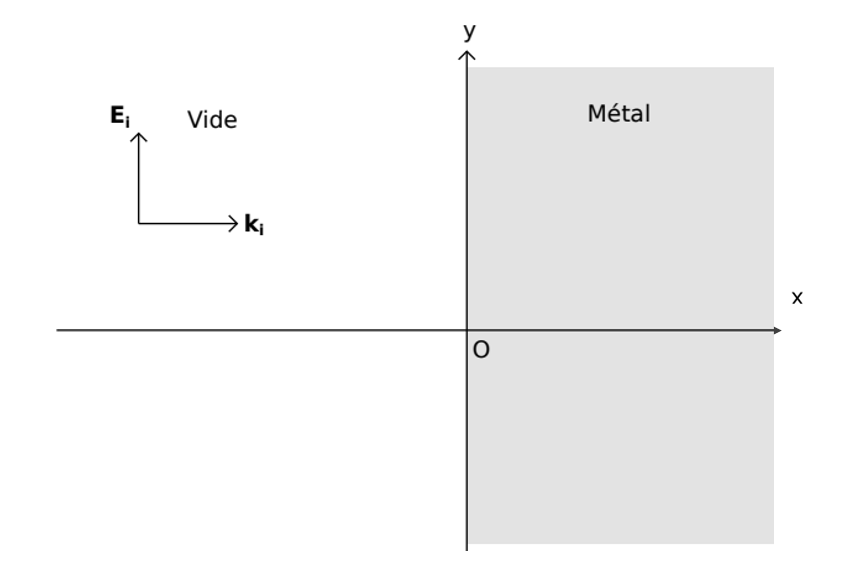
\includegraphics[width=0.4\textwidth]{schéma.png}
  \label{fig:monlabel}
    \caption{Schéma du fil quantique}
\end{figure}

La fonction d’onde propre qui représente alors un état stationnaire d’un électron, d’énergie
$E$, dans le fil s’écrit sous la forme suivante :
$\phi(x) = Aexp(ikx)$
où $A$ est une constante de normalisation réelle. 
\begin{enumerate}
  \item
  \begin{enumerate}
  \item Normaliser la fonction d’onde propre. 
  \item En utilisant l’équation de Schrödinger indépendante du temps, exprimer l’énergie $E$ de
  l’électron en fonction de $k$, $m$ et $\hbar$ Exprimer la vitesse de déplacement $v_xx$, d’un électron selon
  $(Ox)$ en fonction de $k$, $\hbar$ $m$.
  \end{enumerate}
  \item 
  \begin{enumerate} 
    \item Montrer que la densité de probabilité de présence de l’électron $\frac{dP(x)}{dx}$ est uniforme le
  long du fil et donner son expression.
  \item On admet que la probabilité de présence entre $x$ et$ x + dx$, d’un électron, dont le vecteur d'onde est compris entre $k$ et $k+dk$
  est : $dP_k(x)=\frac{dP(x)}{dx}\frac{l}{\pi} dxdk$. Montrer que la contribution au courant électrique qui traverse le fil, dans le sens des $x$ croissant,
  d’un électron dont le vecteur d’onde est compris entre $k $et$ k +dk$ est :
  $dI=-\frac{e v_x}{\pi} dk$, où $e$ désigne la charge élémentaire.
  \end{enumerate}
 \item Le fil quantique est disposé entre deux métaux, soumis à une différence de potentiel électrique
 $U$. La figure suivante représente les niveaux d’énergie des électrons dans les deux métaux.

 
\begin{figure}[h]
  \centering
  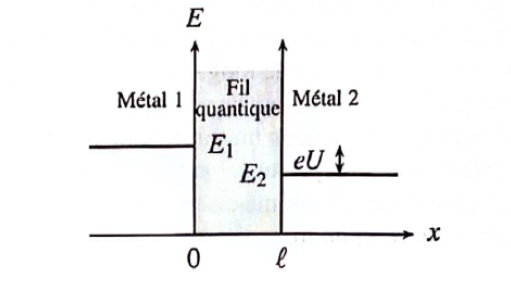
\includegraphics[width=0.4\textwidth]{énergie.png}
  \label{fig:monlabel}
    \caption{Niveaux d'énergie dans les deux métaux.}
\end{figure}
  

Dans le métal 1 du côté $x < 0$, les électrons de conduction occupent tous les niveaux d’énergie
jusqu'à une valeur maximale notée $E_1$; . Dans le métal 2, situé de l’autre côté du fil quantique
($x>0$), les électrons de conduction occupent tous les niveaux d’énergie jusqu’à une valeur
maximale notée $E_2 = E_1 - eU$. Un électron du métal 1 dont l’énergie est comprise entre $E_1$
et $E_2$ peut transiter à travers le fil quantique vers le métal 2. Cet électron a un vecteur d’onde
$k$ compris entre $k_1$ et $k_2$. Les énergies $E_1$ et $E_2$ sont liées à $k_1$ et $k_2$ par la relation déterminée
à la question 1.b.
\begin{enumerate}
  \item Montrer que l'intensité $I$ du courant électrique qui traverse le fil dans le sens des x croissants
  s’exprime en fonction de $U$ sous la forme suivante : $I=-GU$, où G $s’exprime$ simplement
  en fonction de $e$ et de la constante de Planck $h$.
  \item Commenter l’expression de $G$ et donner sa valeur numérique, ainsi que celle de la grandeur
  $R=1/G$.
\end{enumerate}
\end{enumerate}


\section{Mines PC2 2016 }

On traitera les questions 18 à 34. \\[0.5cm]



$\hat{M} = \frac{1}{N} \sum_{i=1}^{N} M(s_i) $,  with $s_i \sim p$

\end{document}


